\documentclass[10pt]{beamer}

\usetheme[progressbar=frametitle]{metropolis}
\usepackage{appendixnumberbeamer}

\usepackage{booktabs}
\usepackage[scale=2]{ccicons}
\usepackage[english]{babel}

\usepackage{pgfplots}

\usepackage{xspace}
\newcommand{\themename}{\textbf{\textsc{metropolis}}\xspace}

\title{UNDERSTANDING \\ DEEP LEARNING REQUIRES \\ RETHINKING GENERALIZATION}
\date{Feb 21 2018}

\author[shortname]{ Aldo Lamarre \inst{1} \and Matthew C.~Scicluna \inst{2}}
\institute[shortinst]{
\inst{1} D\'epartement d'Informatique et de Recherche Op\'erationnelle\\ Universit\'e de Montr\'eal \and %
\inst{2} Montr\'eal Institute of Learning Algorithms\\
Universit\'e de Montr\'eal}
\titlegraphic{\hfill
\includegraphics[height=1.5cm]{MILA.png}}

\begin{document}
	
	\maketitle
	
	\begin{frame}{Table of contents}
		\setbeamertemplate{section in toc}[sections numbered]
		\tableofcontents[hideallsubsections]
	\end{frame}
	
\section{Introduction}

\begin{frame}{Questions}
	\begin{center}
		\textbf{Main Question}\\
		What distinguishes Neural Networks that generalize well from those that don't?
	\end{center}
	\begin{itemize}
		\item Capacity ?
		\item Regularization ?
		\item How we train the model?
	\end{itemize}
	
\end{frame}	

\begin{frame}{Questions}
	
	\begin{figure}
	\centering
		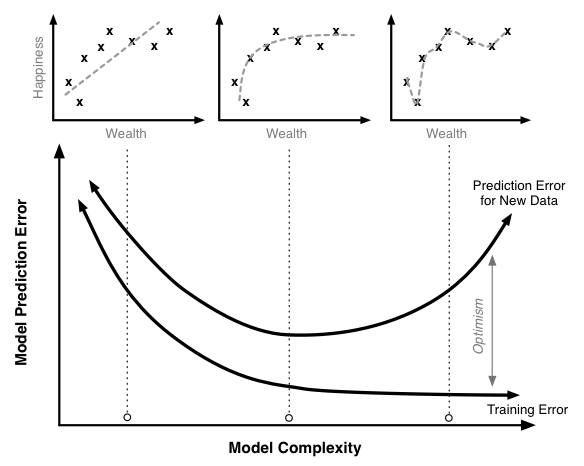
\includegraphics[width=0.7\linewidth]{complexity}
	\caption{Traditional view of generalization. Image taken from \cite{img1}}
	\label{fig:complexity}
	\end{figure}

\end{frame}	

\begin{frame}{Motivation}
\begin{center}
	Why do we care about the problem?
\end{center}
\begin{itemize}
	\item Make neural networks more interpretable
	\item May lead to more principled and reliable model architecture design
\end{itemize}


\end{frame}	

\section{Background}

\begin{frame}{Previous Approaches}
	
Statistical Learning Theory gives bounds on the Generalization Error using:
\begin{itemize}
	\item VC Dimension 
	\item Rademacher Complexity
	\item Uniform Stability
\end{itemize}
Theory suggests that some regularization helps (including Early Stopping)
\end{frame}	

\begin{frame}{Related Work}

In 2016 Hardt et al. gives an Upper bound on Generalization error on model using SGD using uniform stability \cite{DBLP:journals/corr/HardtRS15}

\textbf{BUT}

Uniform stability is a property of a learning algorithm and is not affected by the labelling of the training data.

\end{frame}

\begin{frame}{Limitations}
\begin{alertblock}{Main Message}
	Statistical Learning Theory is insufficient in that it cannot distinguish between neural networks with dramatically different generalization performance.
\end{alertblock}

This is demonstrated in the paper \cite{DBLP:journals/corr/ZhangBHRV16}. The central finding:

\begin{center}
	\emph{Deep neural networks easily fit random labels}
\end{center}

\end{frame}	

\section{Results}

\begin{frame}{Experiment}
	\textbf{Setup}: trained several standard architectures on the data with various modifications:
	\begin{enumerate}
		\item True labels $\rightarrow$ No modifications
		\item Random labels $\rightarrow$ randomly changed some labels
		\item shuffled pixels $\rightarrow$ apply some fixed permutation of pixels to all images
		\item Random pixels $\rightarrow$ apply some random permutation of pixels to all images
		\item Gaussian $\rightarrow$ Generate pixels for all images from a Gaussian
	\end{enumerate}

\end{frame}

\begin{frame}{Main Results}
		\begin{figure}
			\centering
		\centering
		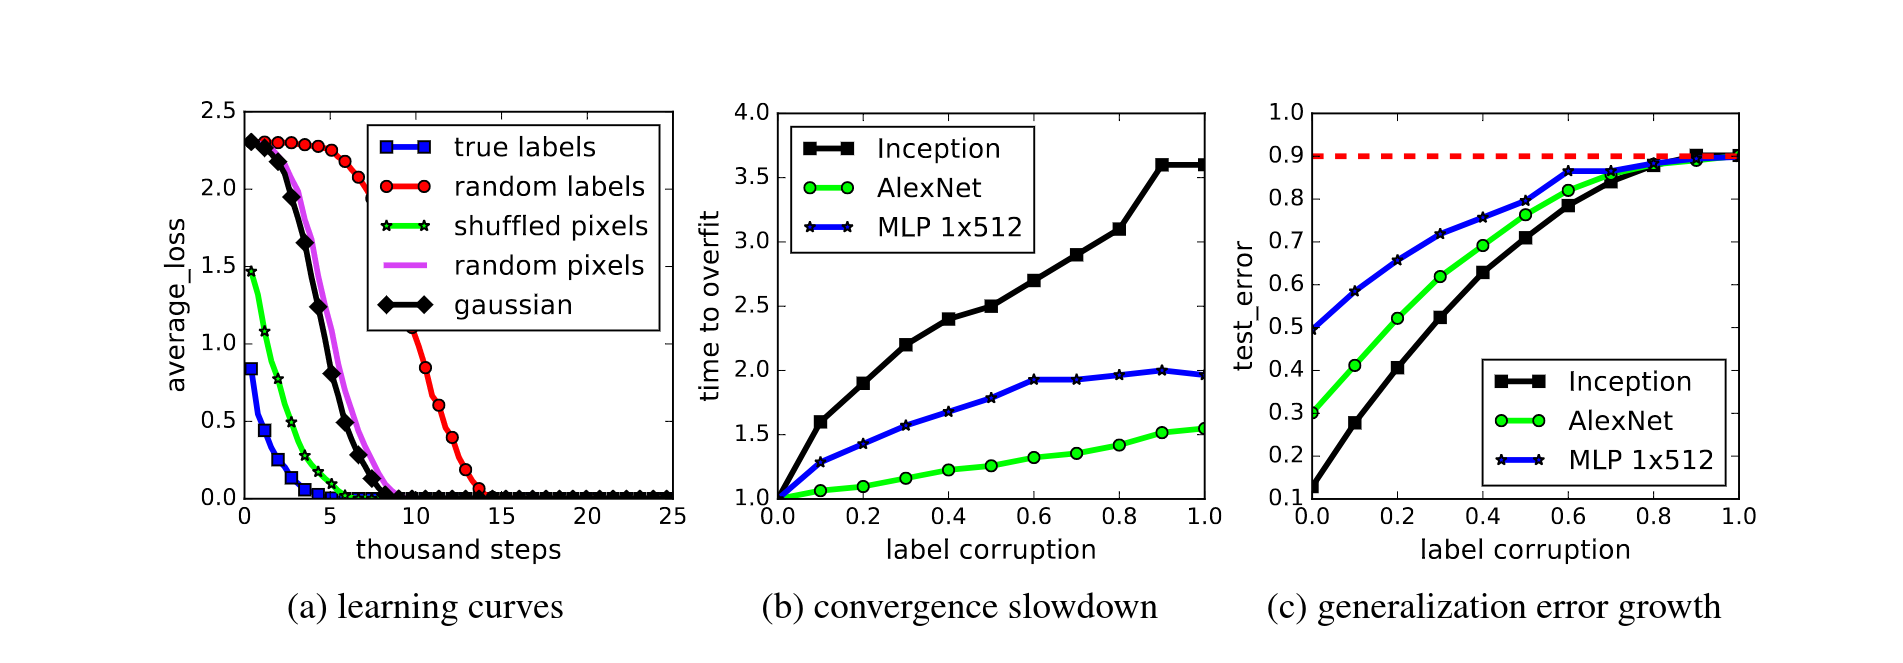
\includegraphics[width=\linewidth]{fig1c}
		\caption{Fitting random labels and random pixels on CIFAR10.}
		\label{fig:corruptlabels}
		\end{figure}
\end{frame}

\begin{frame}{Results}
	In most cases, the training error went to zero while test error was high
	
	\begin{alertblock}{Notice:}
		\emph{the model capacity, hyperparameters, and the optimizer remained the same!}
	\end{alertblock}

\end{frame}

\begin{frame}{Results}
	\begin{center}
			\emph{Explicit regularization may improve generalization performance, but is neither necessary nor by itself sufficient for controlling generalization error}
	\end{center}

	\begin{figure}
		\centering
		\centering
		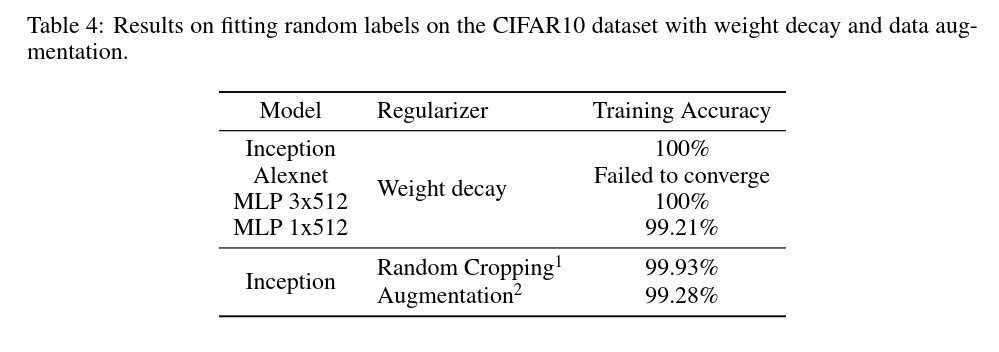
\includegraphics[width=\linewidth]{fig2c}
		\label{fig:withreg}
	\end{figure}
\end{frame}

\section{Technical dive}

\begin{frame}{Technical dive }
	Some definitions:
	\begin{itemize}
		\item \textbf{Representational Capacity}: A models ability to fit a wide variety of functions:
		\item \textbf{Effective Capacity}: The functions that the Learning Algorithm is capable of learning e.g. imperfection of optimization algorithm.
	\end{itemize}
\end{frame}	

\begin{frame}{Finite-sample expressivity }
%Theorem 1.
\begin{block}{Theorem}
There exists a two-layer neural network with ReLU activations and $2n+d$
weights that can represent any function on a sample of size $n$ in $d$ dimensions.
\end{block}
\end{frame}	
\begin{frame}{Proof }
\begin{block}{Lemma 1}
For any two interleaving sequences of n real numbers $b_1 < x_1 < b_2 < x_2 \dots < b_n < x_n$
, the $n \times n$ matrix $A = [max \{x_i - b_j,0\}]_ij$ has full rank. Its smallest eigenvalue is
$min_i\{ x_i - b_i\}$
\end{block}

	%What is an interesting analytical technique, proof method, experimental protocol, other approach to doing things? What is one technical thing that we can learn here? Explain in a few slides.
	
	
\end{frame}	
\begin{frame}{Proof}
%Theorem 1.
For weight vectors $w, b \in R^n$ and $a \in R^d$, consider the function $c : R^n \to R$,
\[c(x) =\sum \limits_{j=1}w_j\, max\{a^Tx - bj , 0\}\]
\only<2->{
\begin{itemize}
\item \only<2>{ This can be done trivially with a depth 2 neural network with relu. }

\only<3,5>{Now, fixing a sample $S = {z_1, \dots , z_n}$ of size n and a target vector $y \in  R_n$. We
	need to find weights $a, b,w $ so that $y_i = c(z_i)$ for all $i \in \{1, \dots , n\}$
}
\only<4>{ First, choose a and b such that with $x_i = a_i^Tz_i$ we have the interleaving property $b_1 < x_1 < b_2 <
	\dots < b_n < x_n$ %This is possible since all zi’s are distinct. 
	Next, consider the set of n equations in the $n$ unknowns $w$, \[y_i = c(z_i) , i \in \{1, \dots , n\}\]
	We have $c(z_i) = Aw$, where $A = [max\{x_i − b_i, 0\}]_{ij}$ is the matrix of Lemma 1.}
\only<5>{\item We chose $a$ and $b$ so that the lemma applies and hence $A$ has full rank. We can now solve the linear
	system $y = Aw$ to find suitable weights w.}
\end{itemize}
}

\end{frame}	
\section{Discussion}

\begin{frame}{Some Thoughts... }
	\begin{enumerate}
		\item Our favourite papers are the ones that shed light on truths that are taken for granted.
		\item Its obvious that randomizing the labels would eliminate generalizability, but explaining why is not!
		\item The paper doesn't really make many conclusions of its own.
		\item The most important result is that a depth 2 neural network with relu activation can learn well overlearn any function.
		\item This result is the most promising to improve with says a test set and other technique to prevent simply learning every point.
	\end{enumerate}

	
	
	%What is not convincing? (too strong assumptions? results not as ‘good’/‘tight’ as other approaches we might know? results are not applicable for ‘x’ reason? bounds are vacuous?)
	
	%What can be improved? (if you where to work in this area, which part of the result would you tweak to make it better, non-vacuous, tighter, more relevant...)
	
	%What interesting open questions that might have been outside the scope of this paper come to your mind when studying it?
\end{frame}	

\begin{frame}{References}
\bibliography{presentation}
\bibliographystyle{ieeetr}
\end{frame}	
	
\end{document}



%\documentclass{beamer}
%
%\mode<presentation>
%{
%	\usetheme{Warsaw}
%	
%	\setbeamercovered{transparent}
%}
%
%\usepackage[utf8]{inputenc}
%\usepackage[english]{babel}
%\usepackage{times}
%\usepackage[T1]{fontenc}
%
%
%
%\institute[University of Toronto] % (optional, but mostly needed)
%{
%	Department of Statistical Sciences\\
%	University of Toronto
%}
%
%\title[UNDERSTANDING DEEP LEARNING REQUIRES RETHINKING GENERALIZATION] % (optional, use only with long paper titles)
%{IFT6085 Paper Presentation}
%
%\subtitle
%{UNDERSTANDING DEEP LEARNING} % (optional)
%
%\author[Aldo Lamarre, Matthew Scicluna] % (optional, use only with lots of authors)
%{~Matthew Scicluna}
%
%\institute[University of Toronto] % (optional, but mostly needed)
%{
%	Department of Statistical Sciences\\
%	University of Toronto
%}
%
%\date[Feb 21 2018] % (optional)
%{Feb 21 2018}
%
%\pgfdeclareimage[height=0.7cm]{university-logo}{MILA.png}
%\logo{\pgfuseimage{university-logo}}
%
%
%
%% Delete this, if you do not want the table of contents to pop up at
%% the beginning of each subsection:
%\AtBeginSubsection[]
%{
%	\begin{frame}<beamer>{Outline}
%		\tableofcontents[currentsection,currentsubsection]
%	\end{frame}
%}
%
%
%% If you wish to uncover everything in a step-wise fashion, uncomment
%% the following command: 
%
%%\beamerdefaultoverlayspecification{<+->}
%
%\begin{document}
%
%\frame{\titlepage}
%
%\begin{frame}
%	\frametitle{What Doesn't Work}
%	\begin{enumerate}
%		\item 
%	\end{enumerate}
%\end{frame}
%
%\begin{frame}
%	\frametitle{Summary}
%	\begin{enumerate}
%		\item Deep neural Networks generalize well
%		\item Conventional wisdom attributes this to properties of the model family or to the regularization techniques used during training
%		\item Experiments show that this is not the case
%	\end{enumerate}
%\end{frame}
%
%\begin{frame}
%	\frametitle{The Experiment}
%	\begin{enumerate}
%		\item Trained state-of-the-art model with SGD on image classification task
%		\item ... with the labels randomly swapped!
%		\item ``easily" fits this training data
%		\item this is qualitatively unaffected by explicit regularization
%		\item and occurs even if we replace the true images with completely unstructured random noise 
%	\end{enumerate}
%\end{frame}
%
%\begin{frame}
%	\frametitle{Introduction}
%	\begin{enumerate}
%		\item What causes Deep artificial Neural Networks to generalize well?
%		\item Statistical Learning Theory gives bounds on generalization error
%		\item Deep neural networks easily fit random labels
%		\item Can make training error 0 while test error is no better then random chance
%	\end{enumerate}
%\end{frame}
%
%\begin{frame}
%	\frametitle{Consequences}
%	\begin{enumerate}
%		 \item The effective capacity of neural networks is sufficient for memorizing the entire data set. 
%		 \item Even optimization on random labels remains easy. In fact, training time increases only by a small constant factor compared with training on the true labels.
%		 \item Randomizing labels is solely a data transformation, leaving all other properties of the learning problem unchanged.
%	\end{enumerate}
%\end{frame}
%
%\end{document}
